\documentclass{beamer}
\usepackage[utf8]{inputenc}
\usepackage[T2A]{fontenc}
\usepackage[english,russian]{babel}
\usepackage{graphicx} % Пакет для работы с изображениями
\usepackage{adjustbox} % Hyperlinks
\usepackage{courier}
\usepackage{blindtext}

\usepackage{float}
\usepackage{listings}

\definecolor{c}{HTML}{000050}

\usetheme{Warsaw}

\setbeamertemplate{footline}[frame number]
\setbeamertemplate{navigation symbols}{}

\begin{document}

\begingroup
\setbeamertemplate{footline}{}

\begin{frame}
\begin{center}
\Large РАЗРАБОТКА БАЗЫ ДАННЫХ ДЛЯ АВТОМАТИЗАЦИИ РАБОЧЕГО МЕСТА РАЗМЕТЧИКОВ ПАРАЛЛЕЛЬНОГО КОРПУСА ТЕХНИЧЕСКИХ ТЕКСТОВ
\end{center}

\vfill

\begin{minipage}[t]{0.45\textwidth}
    \raggedright
    Выполнил:

    студент 3 курса

    группы ИУ7-64Б

    \makebox[0pt][l]{Рунов Константин Алексеевич}
\end{minipage}
\hfill
\begin{minipage}[t]{0.45\textwidth}
    \raggedleft
    Руководитель:

    \makebox[0pt][r]{Строганов Юрий Владимирович}
\end{minipage}

\vfill

\begin{center}
    Москва, \the\year\ г.
\end{center}
\end{frame}
\endgroup

\begin{frame}
    \frametitle{Цель и задачи}
    Цель: Разработать базу данных для автоматизации рабочего места разметчиков параллельного корпуса технических текстов.

    \vfill

    Задачи:
    \begin{itemize}
        \item Провести анализ предметной области корпусов текстов;
        \item Спроектировать и разработать базу данных, описать ее сущности, ограничения целостности, ролевую модель на уровне базы данных и используемые триггеры;
        \item Разработать приложение для доступа к базе данных;
        \item Исследовать зависимость времени ответа от количества запросов в секунду и сравнить эффективности реализаций приложения с использованием дополнительного кеширования и без него.
    \end{itemize}
\end{frame}

\begin{frame}
    \frametitle{Анализ предметной области}
    % Лингвистические корпуса представляют собой структурированные массивы данных, которые используются для изучения языковых единиц в текстах.
Параллельные корпусы — корпусы, представляющие собой множество текстов-оригиналов, написанных на каком-либо исходном языке, и текстов — переводов этих исходных текстов на один или несколько других языков.
    \vfill
    \centering
    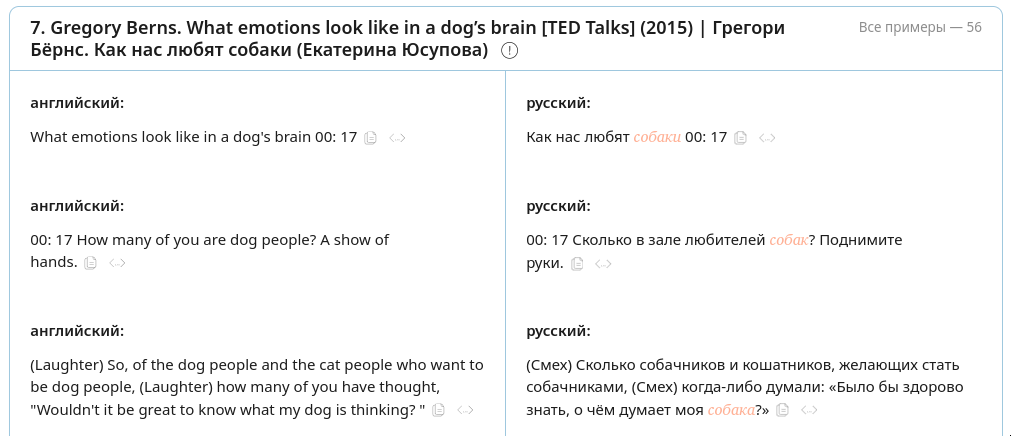
\includegraphics[width=\textwidth]{img/parcor.png}
\end{frame}

% \begin{frame}
%     \frametitle{Анализ предметной области}
%     \centering
%     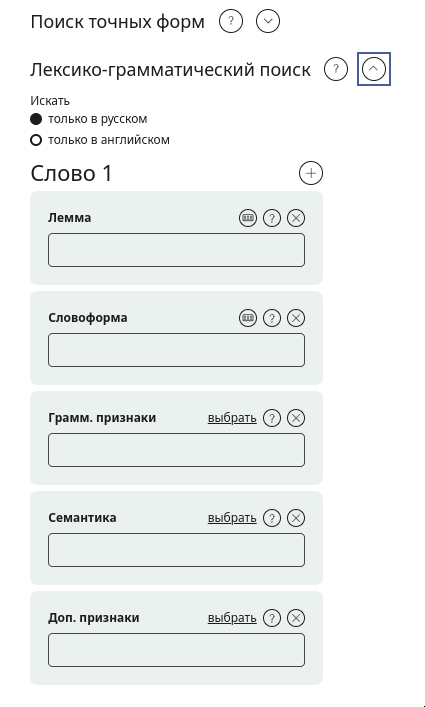
\includegraphics[width=0.45\textwidth]{img/searchcor.png}
% \end{frame}

\begin{frame}
    \frametitle{Анализ предметной области}
    Пример разметки текста в OpenCorpora.
    \vfill
    \centering
    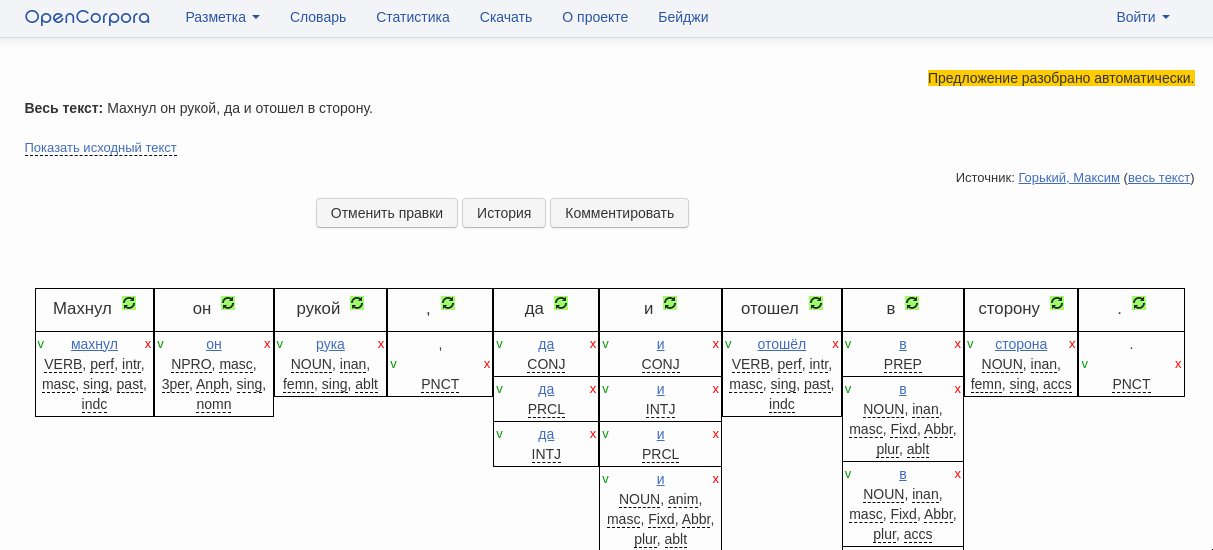
\includegraphics[width=\textwidth]{img/opencorpora.png}
\end{frame}

\begin{frame}
    \frametitle{Существующие аналоги}
    \centering
	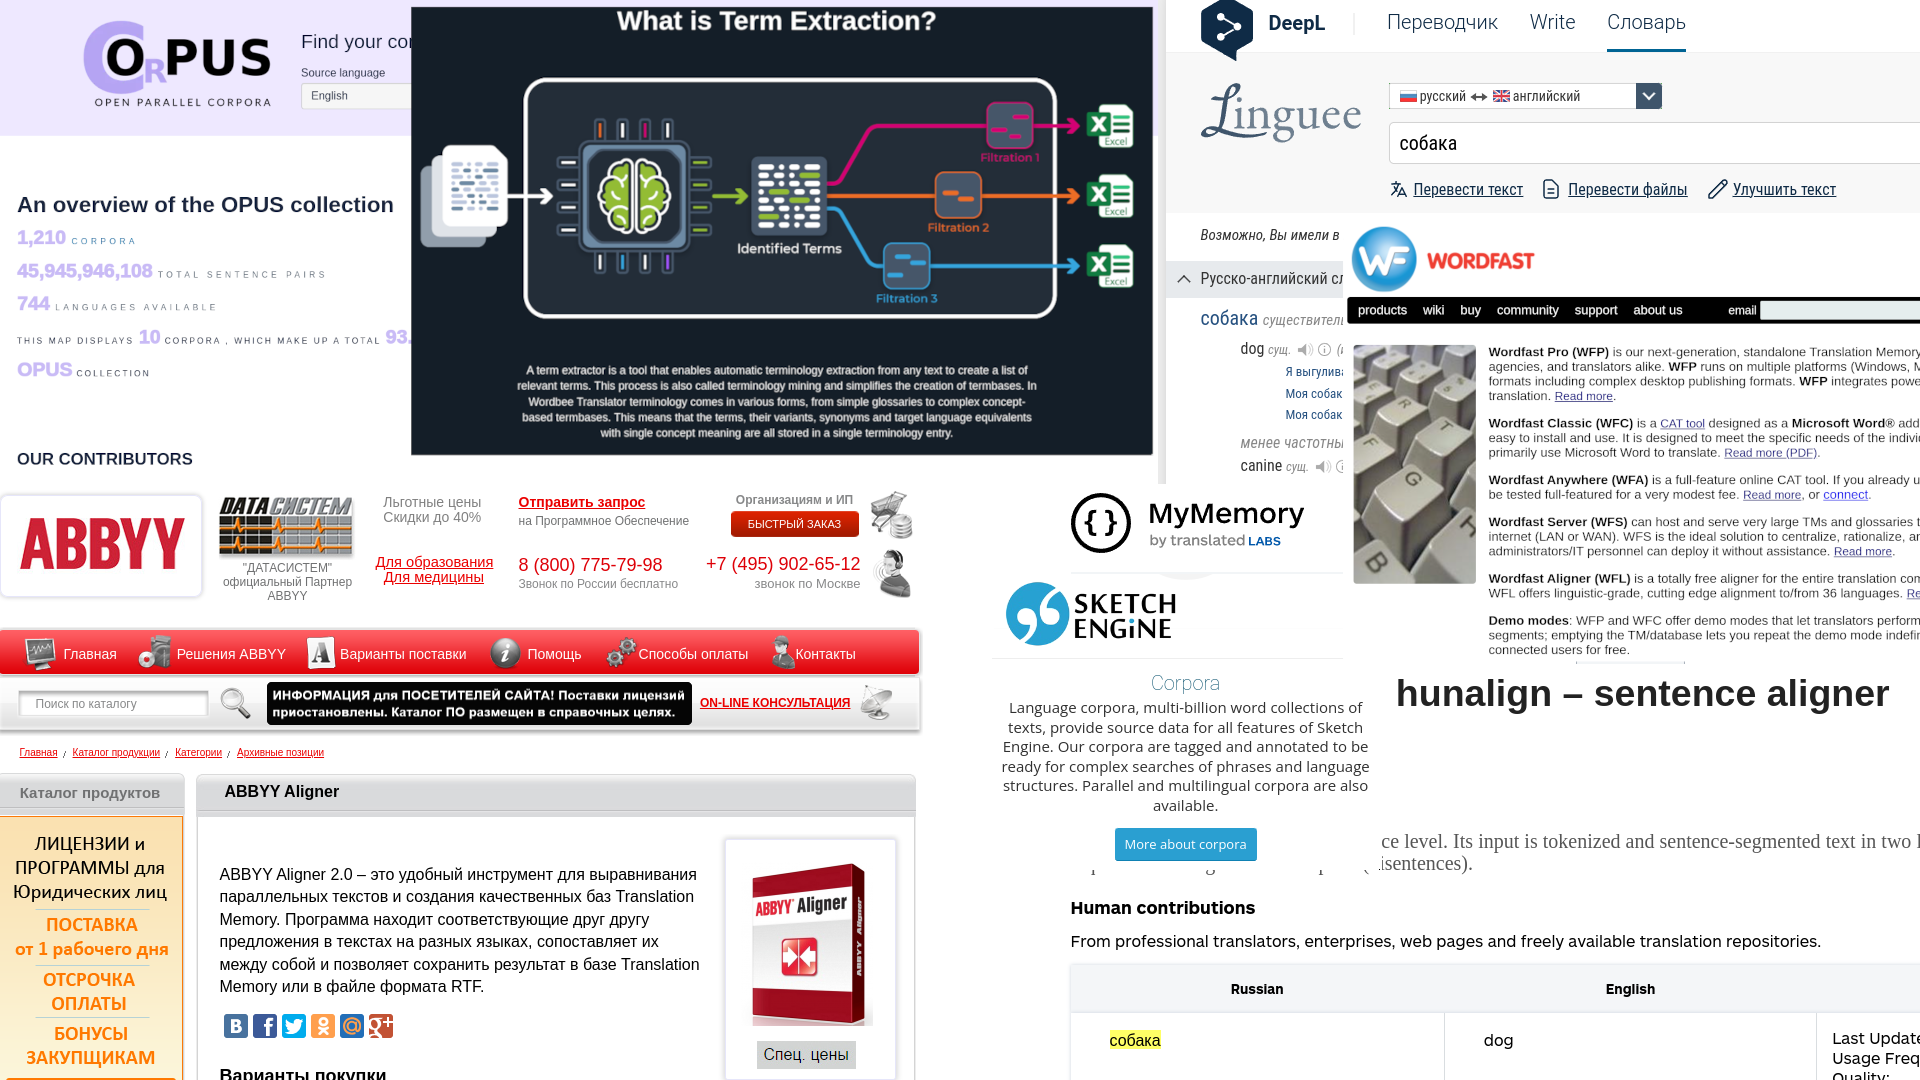
\includegraphics[width=\textwidth]{img/alternatives.png}
\end{frame}

\begin{frame}
    \frametitle{Диаграмма сущностей}
    \centering
	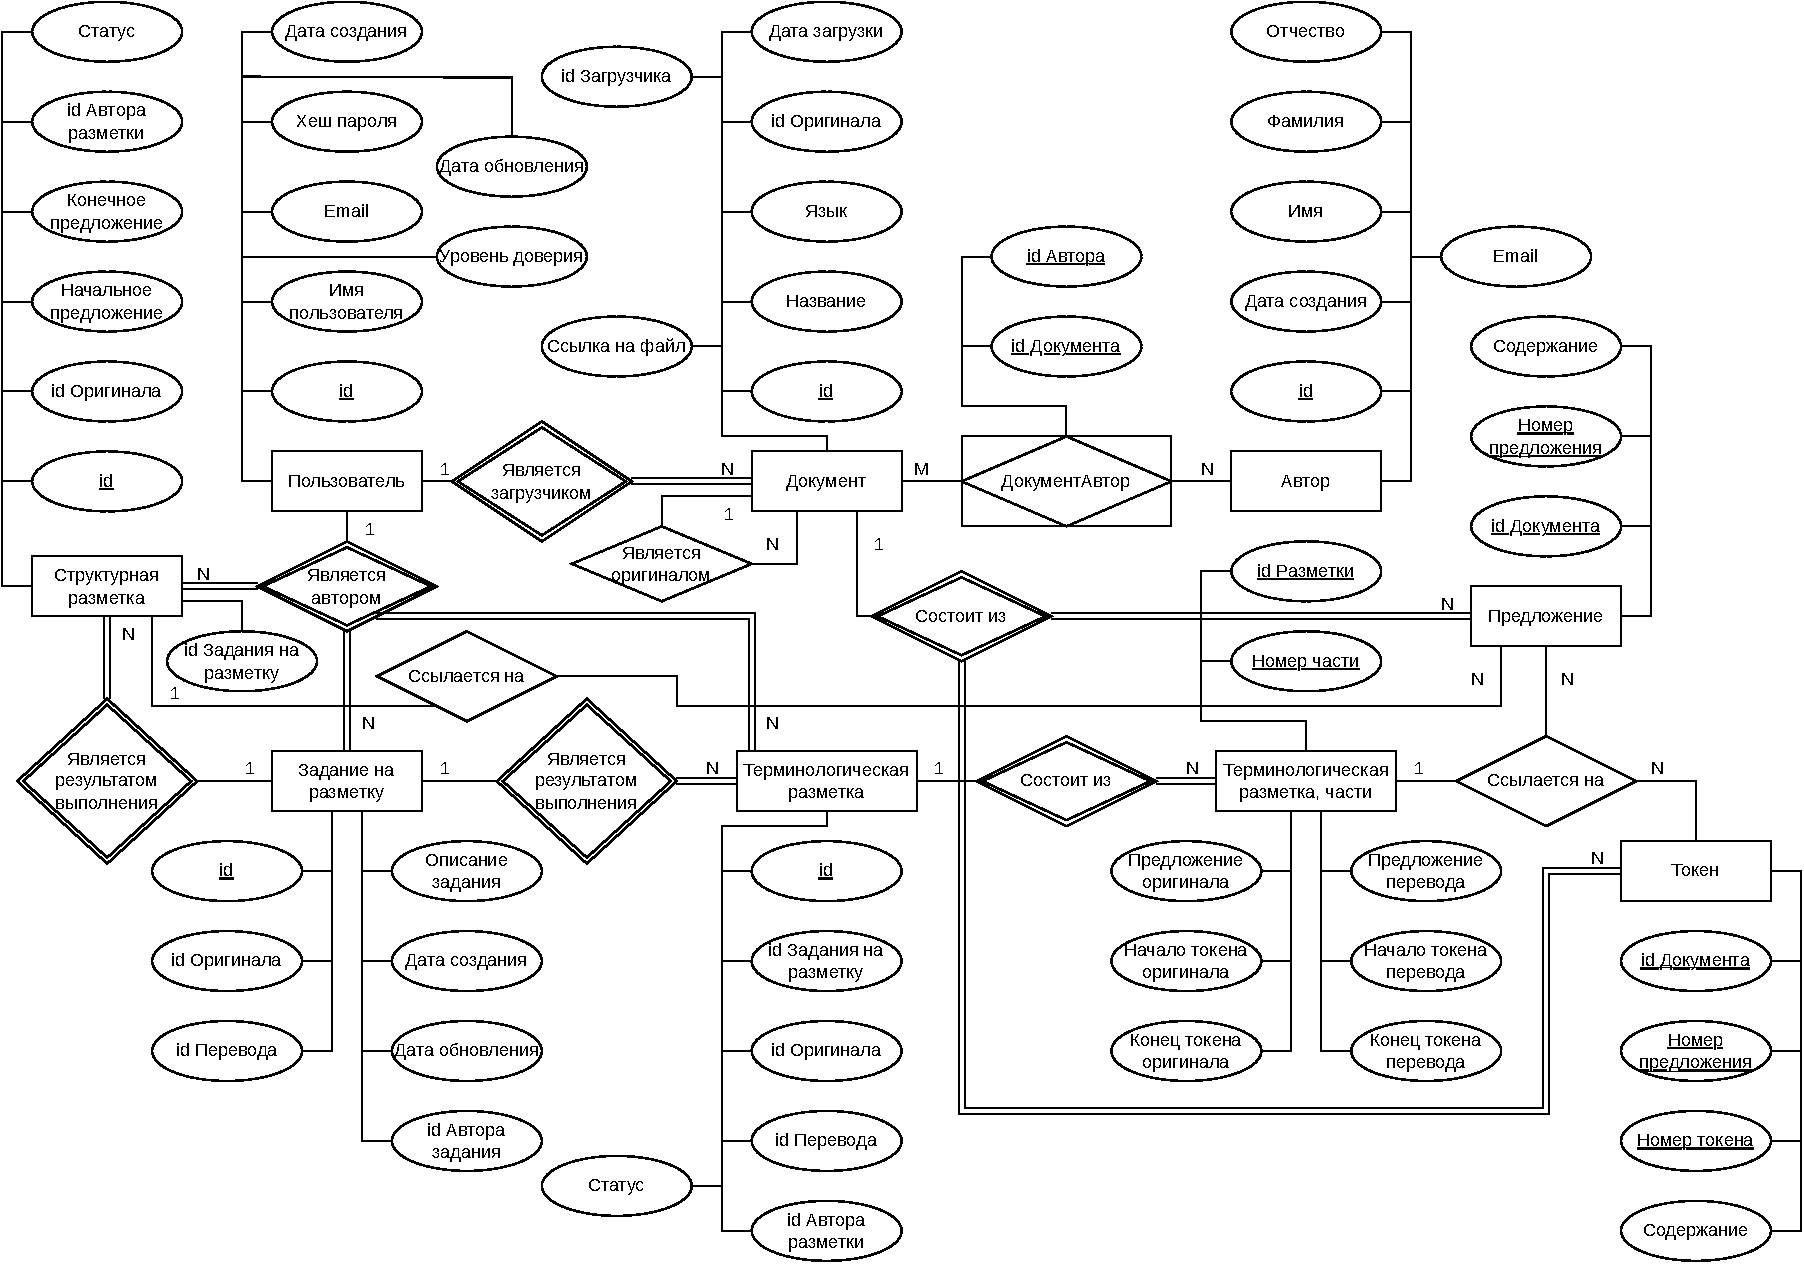
\includegraphics[width=\textwidth]{diag/chen-v9.pdf}
\end{frame}

\begin{frame}
    \frametitle{Диаграмма вариантов использования}
    \begin{itemize}
        \item Администратор имеет полный доступ к данным: может добавлять, удалять и изменять тексты и разметки.
        \item Модераторы создают задания на разметку и производят проверку разметок, осуществленных пользователями.
        \item Пользователи осуществляют разметку и выполняют поиск по корпусу.
    \end{itemize}
    \vfill
    \centering
	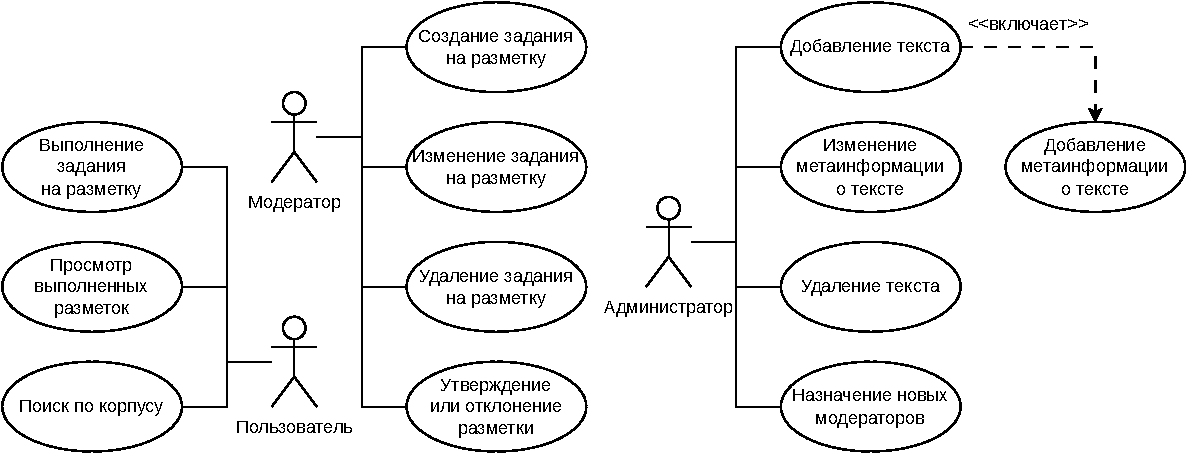
\includegraphics[width=\textwidth]{diag/use-case-v2.pdf}
\end{frame}

\begin{frame}
    \frametitle{Диаграмма проектируемой БД}
    \centering
	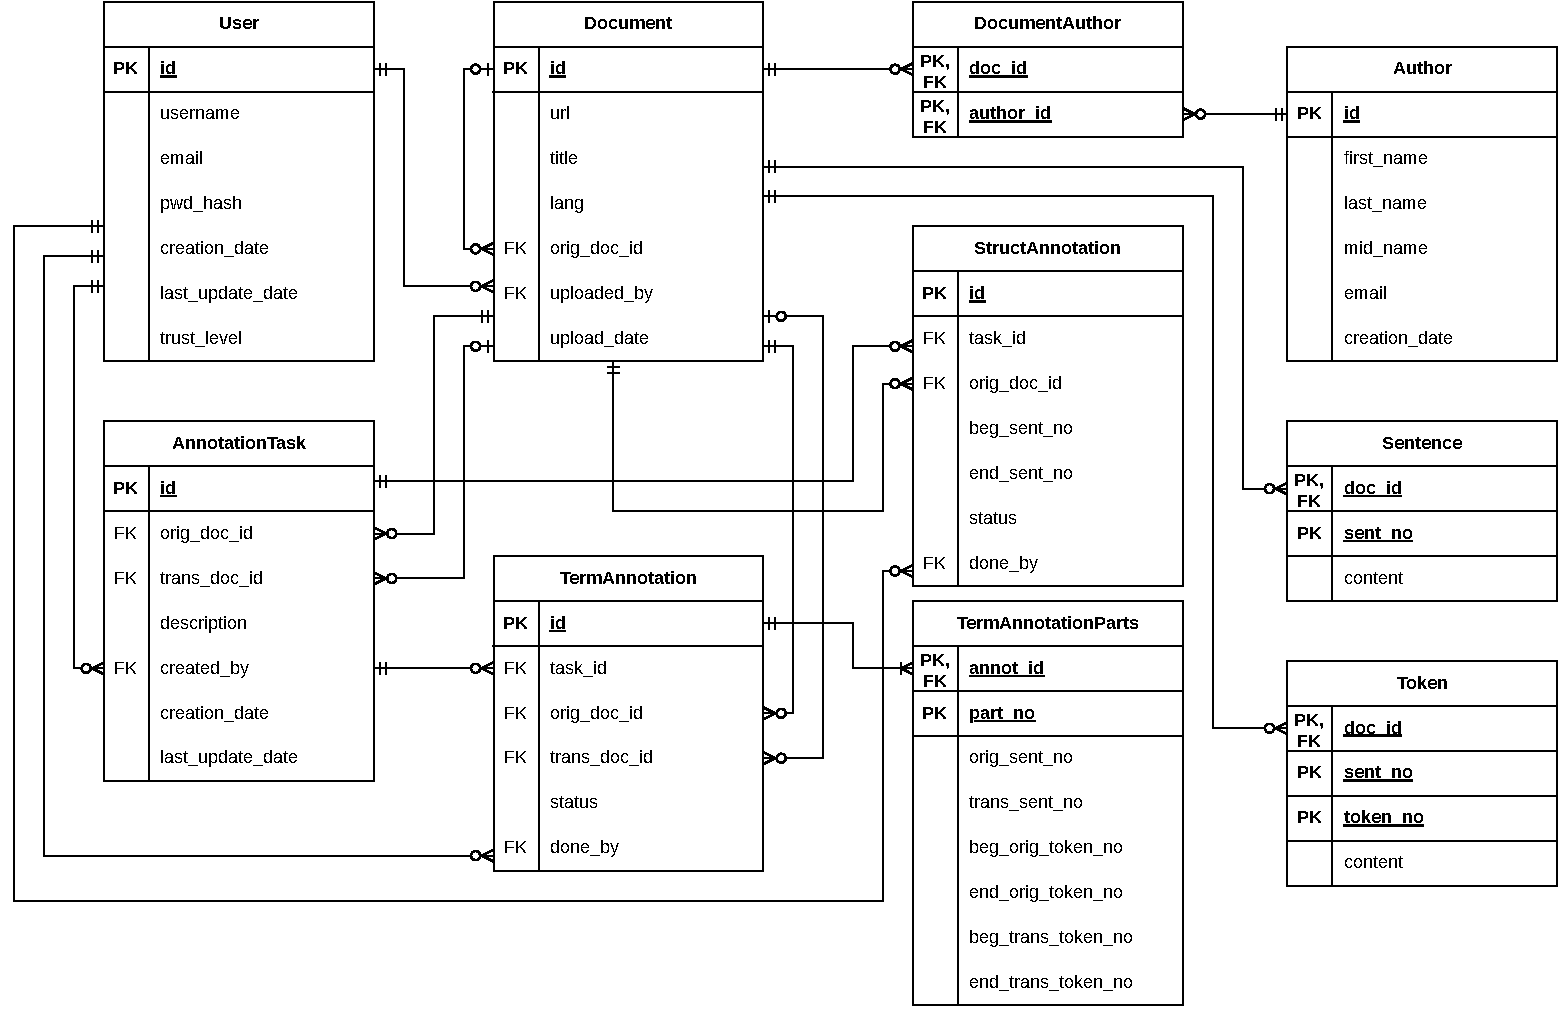
\includegraphics[width=\textwidth]{diag/erd-v3.pdf}
\end{frame}

\begin{frame}
    \frametitle{Схема проектируемого триггера}
    \centering
	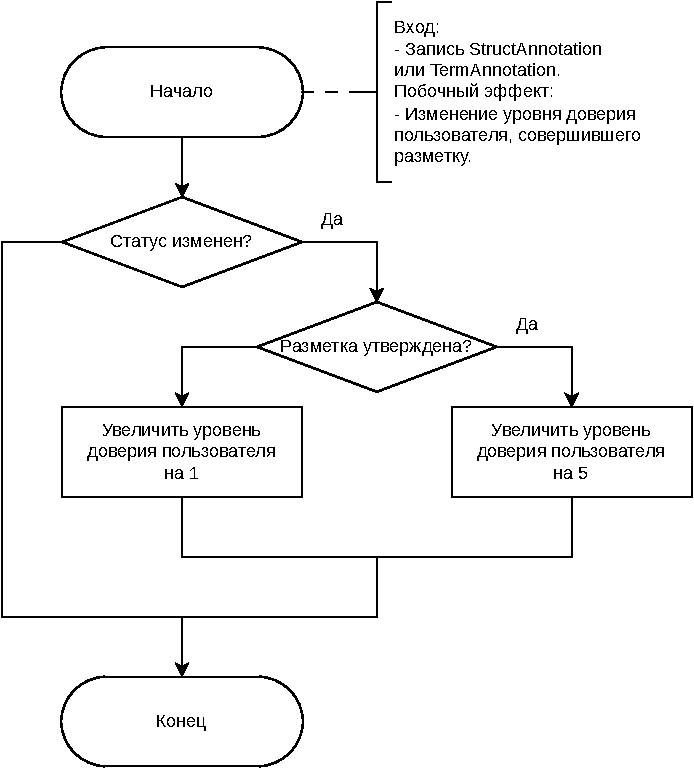
\includegraphics[width=0.6\textwidth]{diag/trig-v4.pdf}
\end{frame}

\begin{frame}
    \frametitle{Выбор СУБД}
    Была выбрана PostgreSQL по следующим причинам:
    \begin{itemize}
        \item Реализует реляционную модель, которая, как было выяснено, является наиболее подходящей для базы данных, разрабатываемой в настоящей работе;
        \item Открытый исходный код;
        \item Поддержка полнотекстового поиска;
        \item Имеется опыт работы с данной СУБД.
    \end{itemize}
\end{frame}

\begin{frame}
    \frametitle{Схема реализованного триггера}
    \centering
	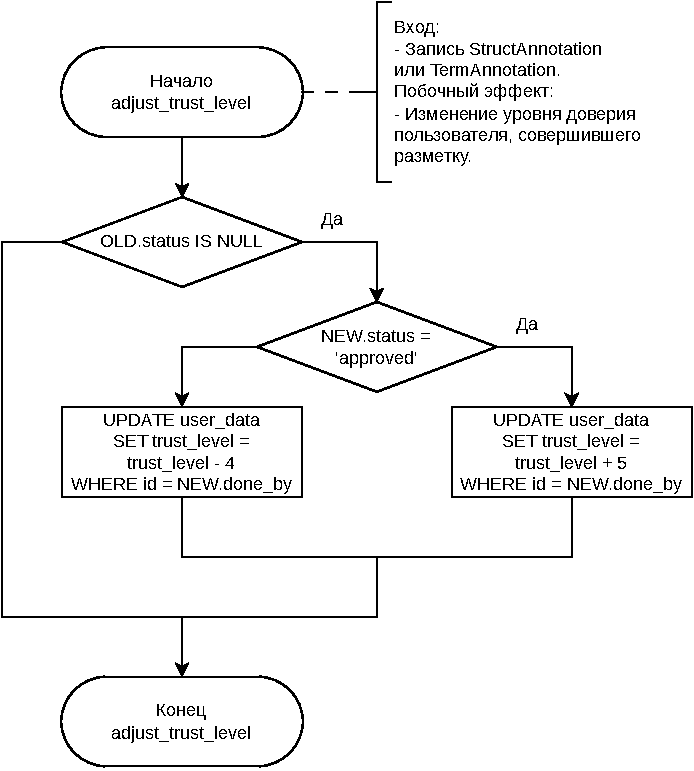
\includegraphics[width=0.6\textwidth]{diag/tech-trig-v4.pdf}
\end{frame}

\begin{frame}
    \frametitle{Проведение исследования, locustfile.py}
    \centering
\lstset{language=Python, morekeywords={self}}
\begin{lstinputlisting}[
    label={lst:},
]{../src/scripts/lf.py}
\end{lstinputlisting}
\end{frame}

\begin{frame}
    \frametitle{Проведение исследования, интерфейс Locust}
    \centering
	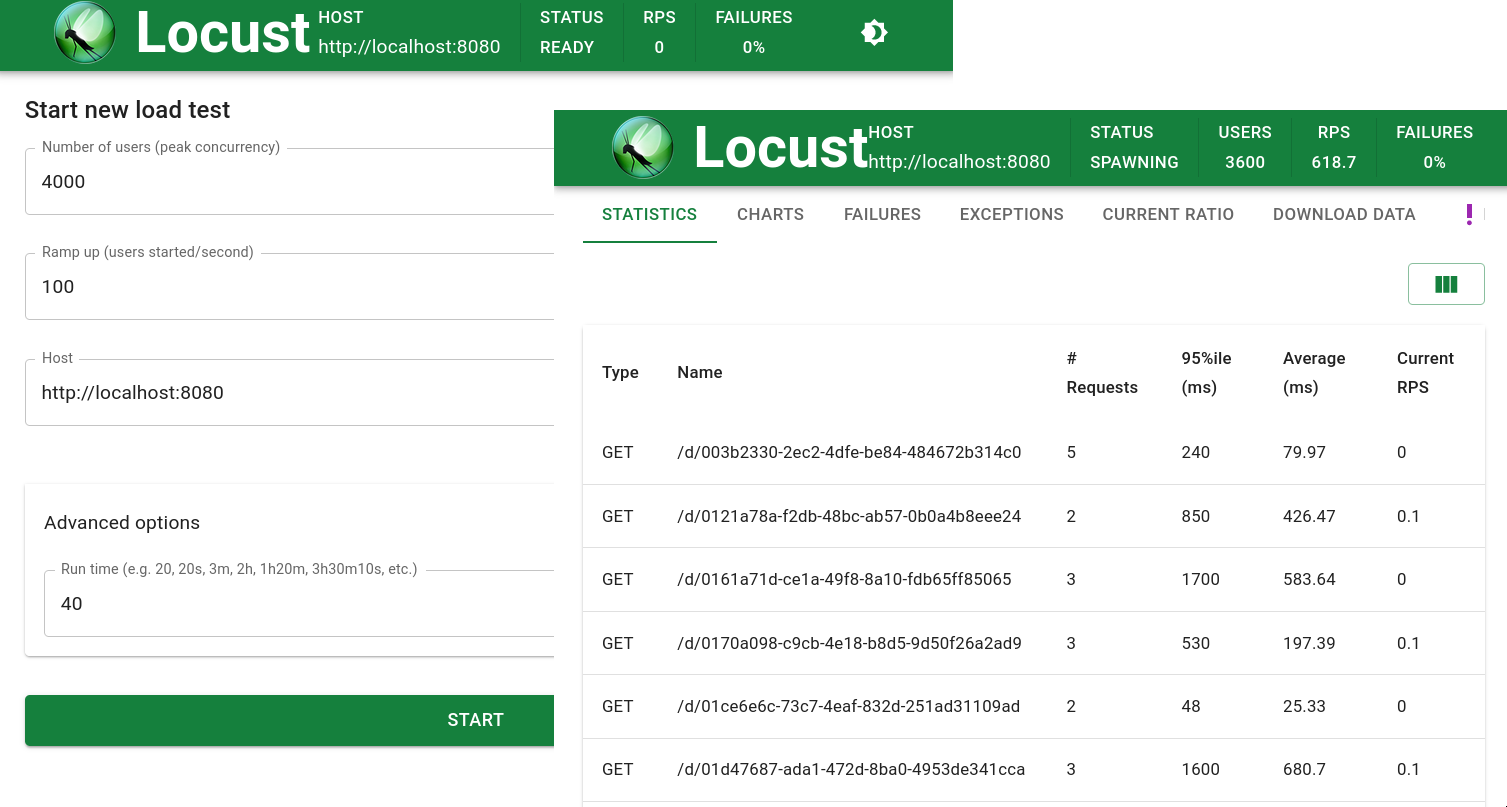
\includegraphics[width=\textwidth]{img/pres-locust-1.png}
\end{frame}

\begin{frame}
    \frametitle{Проведение исследования, интерфейс Locust}
    \centering
	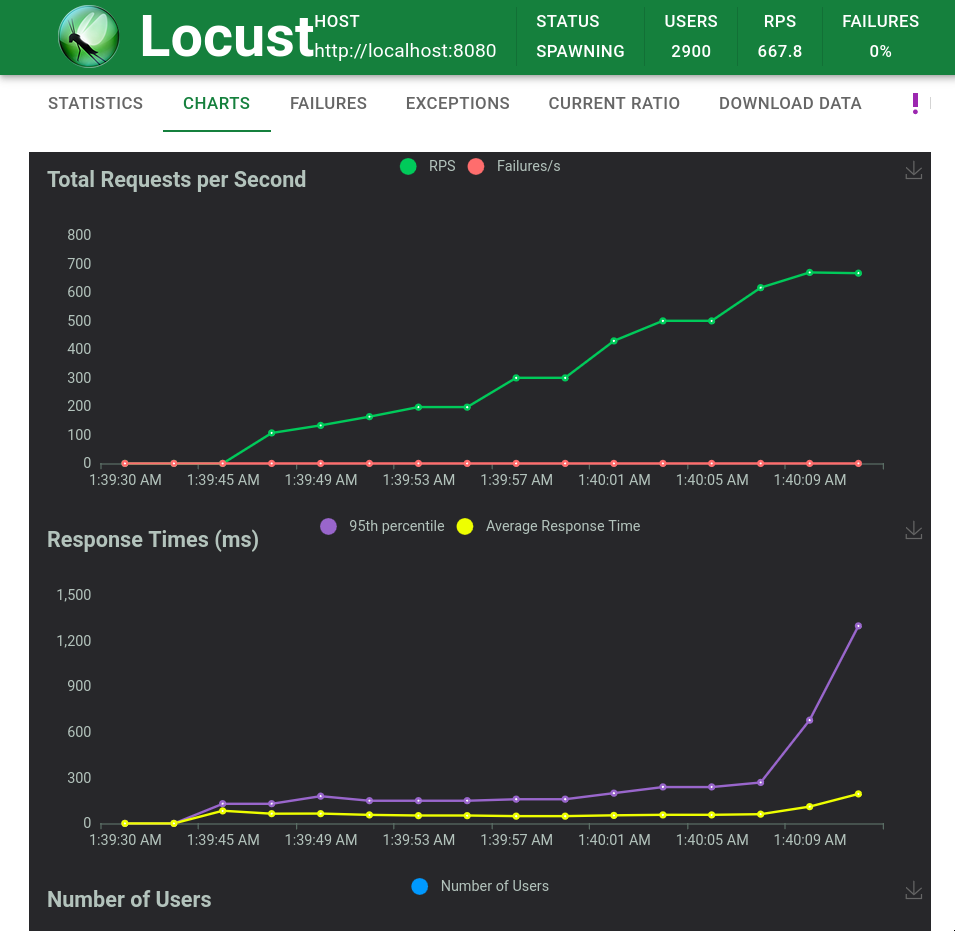
\includegraphics[width=0.8\textwidth]{img/locust-scr-3.png}
\end{frame}

\begin{frame}
    \frametitle{Результаты исследования}
    \centering
    {
        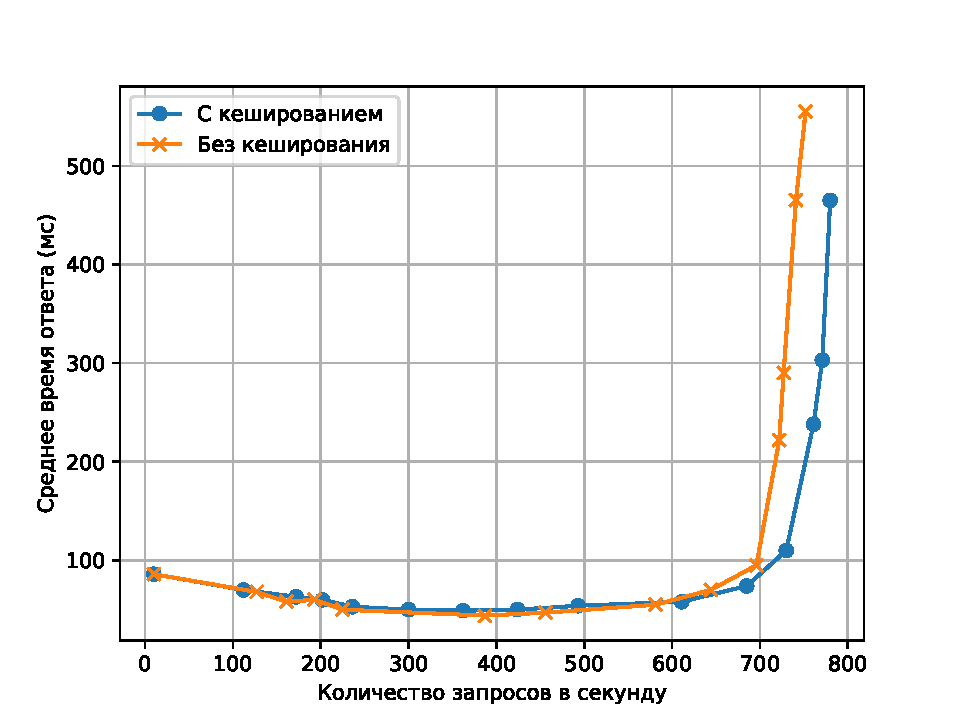
\includegraphics[width=0.9\textwidth]{img/avg-resp-time.pdf}
    }
    \vfill
    При 752 запросах в секунду использование кеша позволило ускорить среднее время ответа более, чем в 3 раза.
\end{frame}

\begin{frame}
    \frametitle{Результаты исследования}
    \centering
    {
        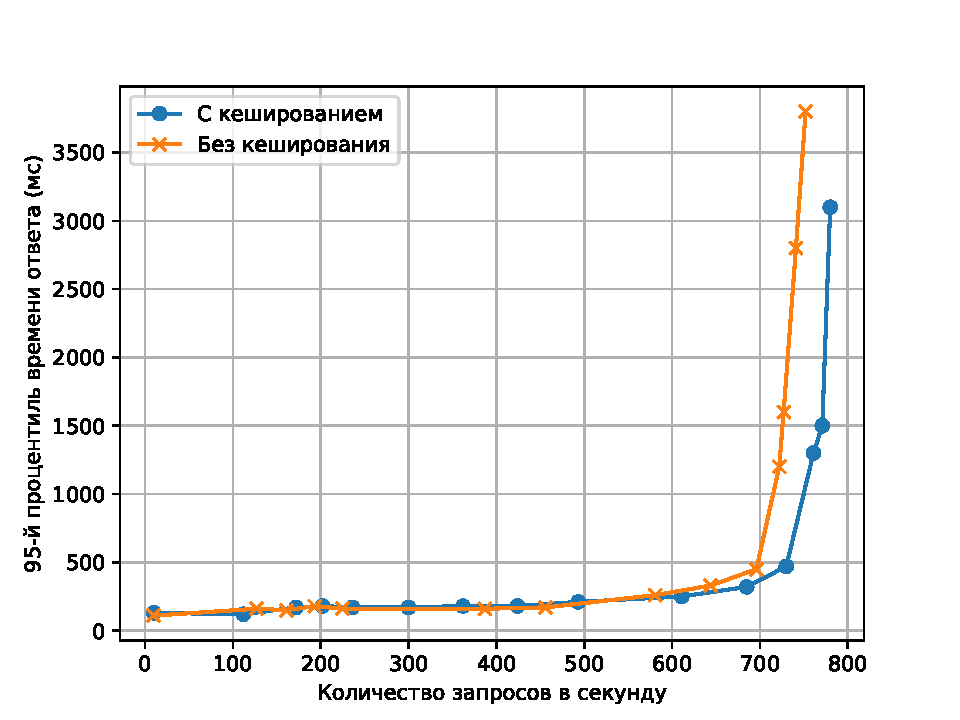
\includegraphics[width=0.9\textwidth]{img/95-resp-time.pdf}
    }
    \vfill
    При 750 запросах в секунду 95 процентов запросов к приложению с кешем обрабатываются в 3.45 раза быстрее.
\end{frame}

\begin{frame}
    \frametitle{Заключение}
    Поставленная цель: Разработка базы данных для автоматизации рабочего места разметчиков параллельного корпуса технических текстов была достигнута.

    \vfill
    Для достижения цели были выполнены поставленные задачи:
    \begin{itemize}
        \item Проведен анализ предметной области корпусов текстов;
        \item Спроектирована и разработана база данных, описаны ее сущности, ограничения целостности, ролевая модель на уровне базы данных и используемые триггеры;
        \item Разработано приложение для доступа к базе данных;
        \item Исследована зависимость времени ответа от количества запросов в секунду.
    \end{itemize}
    \vfill

    В результате исследования было выяснено, что использование кеша позволяет ускорить среднее время ответа более, чем в 3 раза при большом (752) количестве запросов в секунду.
\end{frame}

\begin{frame}
    \frametitle{Направления дальнейшего развития}
    Далее на основе реализованных базы данных и приложения к базе данных можно сделать, например, следующее:
    \begin{itemize}
        \item Добавить поддержку загрузки PDF-документов;
        \item Интегрировать приложение с различными автоматическими выравнивателями и разметчиками;
        \item Разработать приложение --- социальную сеть для разметчиков текстов, в котором разметчики могут оперативно делиться разметками и выполнять задания, повышая свой рейтинг.
    \end{itemize}
\end{frame}

\end{document}
